\chapter{Networking and Cryptography tools} % (fold)
\label{cha:Networking and Cryptography tools}
	Here we describe the networking and cryptographic tools used in this protocol.
	For example, we describe the Hash function, its properties and how it helps us achieve data integrity.

\section{Hash Function}
	A hash function takes a message as its input and outputs a fixed length message called hash code.
	The hash code represents a compact image of the message like a digital fingerprint.
	Hash functions are used to achieve data integrity.

	A hash function $h$ should have the following properties:
	\begin{itemize}
		\item Compression - $h$ maps an input $x$ of arbitrary finite bitlength, to an output $h(x)$ of fixed bitlength $n$.
		\item Ease of computation - given $h,x$ it is easy to compute $h(x)$.
		\item Preimage resistance - for all pre-specified outputs, it is computationally infeasible to find any input which hashes to that output, i.e., to find any preimage $x'$ such that $h(x') = y$ when given $y$ for which a corresponding input is not known.
		\item 2nd-preimage resistance - it is computationally infeasible to find any second input which has the same output as any specified input, i.e, given $x$, to find a 2nd-preimage $x' \neq x$ such that $h(x') = h(x)$.
		\item Collision resistance - it is computationally to find any two distinct inputs $x,x'$ which hash to the same output, i.e., such that $h(x) = h(x')$.
	\end{itemize} 

	We use SHA-$256$\cite{SHA256} hash algorithm as a hash algorithm.
	% cite NIST for SHA-256

\section{Digital Signatures}
	A digital signature is a mathematical scheme for demonstrating the authenticity of a digital message. 
	A valid digital signature gives a recipient reason to believe that the message was created by a known sender, such that the sender cannot deny having sent the message (authentication and non-repudiation) and that the message was not altered in transit (integrity).
	A Digital Signature scheme consists of the following:
	\begin{enumerate}
		\item a plain text message space $\mathcal{M}$ (set of strings over alphabets)
		\item a signature space $\mathcal{S}$ (set of possible signatures)
		\item a signing key space $\mathcal{K}$ (set of possible keys for signature generation) and a verification space $\mathcal{K^{'}}$ (a set of possible verification keys)
		\item an efficient key generation algorithm \textsf{Gen} : $N \rightarrow$ $\mathcal{K} \times \mathcal{K^{'}} $ 
		\item an efficient signing algorithm \textsf{Sign} : $ \mathcal{M} \times \mathcal{K} \rightarrow \mathcal{S}$
		\item an efficient verification algorithm \textsf{Verify} : $\mathcal{S} \times \mathcal{M} \rightarrow$ \{true, false\} 
	\end{enumerate}
	\textcolor{red}{cite Book for slides}\\
	For any secret key $s_{k} \in \mathcal{K}$ and any $m \in \mathcal{M}$,	the message $m$ is signed using key $s_{k}$ as follows:
		\begin{equation}
			s = \textsf{Sign}_{s_{k}}(m)
			\label{eq:signature}
		\end{equation}
	For any $s_{k}$ let $p_{k}$ denote public key and for all $m \in \mathcal{M}$ and $s \in \mathcal{S}$, $s$ as follows:
	\begin{equation}
		\textsf{Verify}_{p_{k}}(m,s) = 
		\begin{cases}
		 \textbf{true}\ \mbox{with probability of 1} & if\ s = \textsf{Sign}_{s_{k}}(m)\\
		 \textbf{false}\ \mbox{with overwhelming probability} & if\ s \neq \textsf{Sign}_{s_{k}}(m)
		\end{cases}
		\label{eq:verification}
	\end{equation}
	where the probability space is determine by the $\mathcal {M, S, K, K^{'}}$ and perhaps the signing and verification algorithms.
	The ``overwhelming probability'' for the signature scheme determines the probability that the scheme allows for a forgery.
	Note that the Digital Signature scheme satisfies the following requirements:
		\begin{itemize}
			\item Only the owner of the secret key can generate a valid signature.
			\item The digital signature is easily verified by other parties.
			\item The digital signature is not only tied to the signer but also to the message that is being signed.
			\item Digital signatures cannot be separated from the message and attached to another message.
			\item Digital signatures do not encrypt the message. However, if necessary, a signed message can be encrypted after it is signed.
		\end{itemize}
	The Figure \ref{fig:digita-signature} from \cite{DigitalSignature}, shows the steps for signing and verifying the hashed message. 
	\begin{figure}[h!]
		\centering
		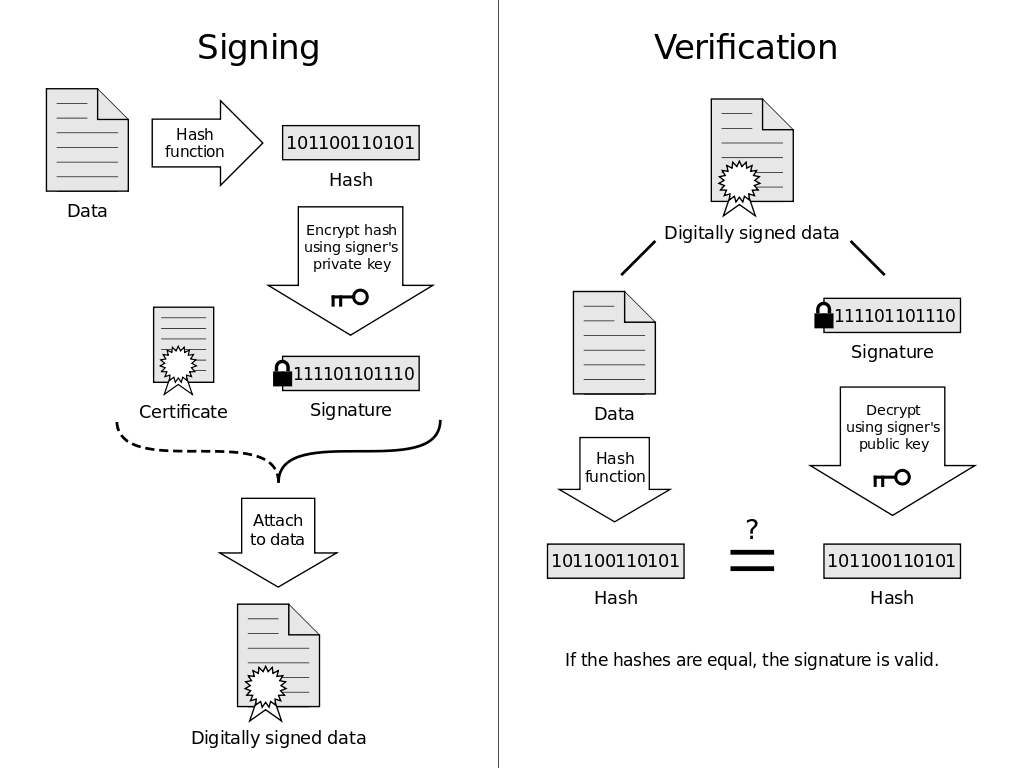
\includegraphics[scale = 0.4]{images/Digital_Signature_diagram.png}
		\caption{ Signing and verification of digital signatures}
		\label{fig:digita-signature}
	\end{figure}
	The message is hashed before its being signed to reduce the message size. 
	If the message is not hashed before signing then the signature can be longer than the message which is problematic for the longer messages.

\section {Tree generation algorithms}


\section{Elliptic curve}